\documentclass[11pt, twocolumn]{article}
\usepackage[utf8]{inputenc}
\usepackage{blindtext}
\usepackage{setspace}
\usepackage{geometry}
\usepackage{graphicx}
\usepackage{mathtools}
\usepackage{unicode-math}
\usepackage{amssymb}
\usepackage{bm}
\usepackage[font={small}]{caption}
\geometry{a4paper, left=10mm,  top=15mm, bottom=22mm, right=10mm}
\usepackage[english]{babel}
\usepackage[sorting=none]{biblatex}
\usepackage{comment}
\setlength{\columnsep}{5mm} 
\addbibresource{bibliography.bib}

\title{Measuring Matter Antimatter Asymmetries at the Large Hadron Collider}
\author{Rutwik Mudholkar 10327919}

\begin{document}
\maketitle

\onehalfspacing
\setlength\parindent{0pt}

\section*{Abstract}
We aim to measure a fundamental difference between the behaviour of
matter and antimatter through the analysis of data collected by LHCb. specifically for the charmless three-body decay of $B^{\pm} \rightarrow K^{\pm}K^{+}K^{-}$. We calculate the matter antimatter asymmetry, and larger asymmetries are searched for in localized regions of the phase-space. We find a negligible global CP asymmetry $A_{CP}$ of $−0.039 \pm 0.013$, and significant local CP violation in the $(0.1\sim0.2) \times 10^7 \ \mathrm{MeV}^2$ two-body resonance mass region.  

\section{Introduction}

Since the big-bang is expected to have produced equal amounts of matter and antimatter, the existence of our matter dominated universe remains one of the major outstanding questions of fundamental physics. The phenomenon of charge-parity (CP) symmetry violation was recognized as one of the requirements, known as the Sakharov conditions, for how this could have arisen \cite{universe}. It was first seen experimentally with weak decays in K meson systems \cite{first}.\newline

A mechanism for CP violation in the Standard Model had prior been suggested through the CKM matrix, and then verified by showing significant CP asymmetry in decays of neutral $B$ mesons to final states containing charmonium \cite{charmonium}. The magnitude of such reactions however is far too small to explain the matter antimatter imbalance in the universe, thus additional sources of CP violation are required. We can therefore search for more asymmetrical $B$ decays, specifically charged and charmless decays to three K mesons. 

\section{Methodology}
We used pre-selected data collected from the LHCb detector \cite{cern}, a single-arm forward spectrometer dedicated to studying CP violation and rare decays of hadrons containing $b$ and $c$ quarks. The $B$ meson decays after travelling a few mm to a cm in the detector, and is reconstructed from its decay products. These products pass through straw drift tubes \cite{straw} ionising the gas inside, and this new charge is drifted under an electric field to be measured. The measured points are used to reconstruct the track of the charged products, from which the momentum is derived. The products charges are calculated from their direction of bending under a magnetic field, which can be binned into $+$ and $-$ due to charge quantisation. Different types of charged hadrons ($\pi, K$) are then distinguished using photon radiation angle information from two ring-imaging Cherenkov detectors \cite{cherenkov} combined with the hadron momentum. These are given as probabilities. For three body decays, data is collected from three decay channels ($H1, H2, H3$).

To obtain pure signal data for our CP Asymmetry ($A_{CP}$) calculations, we remove non-signal noise and background events from our data, and filter any charmed decays. Using
\begin{equation}
    M_{inv} = \sqrt{(E_1 + E_2 + E_3)^2 - (\bm{p}_{H1} + \bm{p}_{H2} + \bm{p}_{H3})^2}
\end{equation}
where 
\begin{equation}
    E_i = \sqrt{\bm{p}_{Hi} \cdot \bm{p}_{Hi} - M_{Hi}^2},  
\end{equation}
we obtain a fitted invariant mass spectrum for $B^{\pm}$. From this we identify signal regions, and subtract noise and background. We then a plot two-body resonance spectrum for high and low mass pairs to identify and cut mass ranges for products containing charmonium, a result of a $b$ quark decaying to a $c$ quark. Using our cleaned data, we calculate global $A_{CP}$ by comparing individual mass plots for $B^{+}$ and $B^{-}$, and local $A_{CP}$ by analysing their Dalitz Plots. We define 
\begin{equation}
    A_{CP} = \frac{N^{-}-N^{+}}{N^{-}+N^{+}}
\end{equation}
where $N^{+}$ is the number of $B^{+} \rightarrow K^{+}K^{+}K^{-}$ events observed and $N^{-}$ the number for the corresponding $B^{-}$ decay. A statistical uncertainty
\begin{equation}
\sigma_{A_{CP}}=\sqrt{\frac{1-A^2}{N^{-}+N^{+}}}
\end{equation}
is derived by modelling $A_{CP}$ as binomially distributed random variable. For all our data analysis, we apply a general Kaon probability filter
\begin{equation}
    P_{H1,2,3}(K) > 0.7,
\end{equation}
to ensure we only include decays to three Kaons, whilst retaining a high number of data points.


\section{Results}
\begin{figure}[htp]
    \centering
    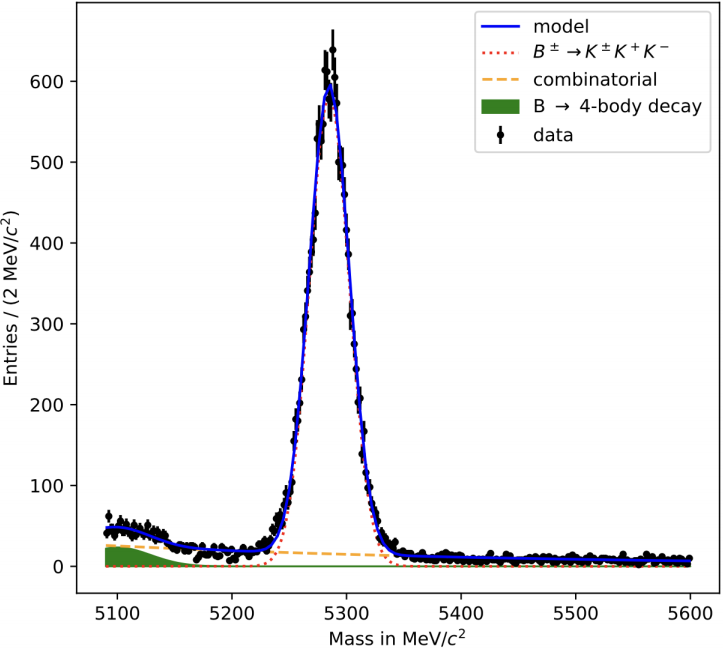
\includegraphics[width=9.2cm]{graph1.png}
    \caption{Invariant mass histogram plot for $B^{\pm} \rightarrow K^{\pm}K^{+}K^{-}$ decays binned at  $2 \ \mathrm{MeV}$. The solid and dotted lines show the best fit curve before and after background and noise removal respectively.}
\end{figure}
Figure 1 shows a signal region approximately the shape of a Gaussian distribution, peaked at $\sim 5280 \ \mathrm{MeV}$. This is consistent with the accepted value of $M_{B^{\pm}} = (5279.34 \pm 0.12) \ \mathrm{MeV}$ \cite{Bplusminus}. We consider the regions outside a $100 \ \mathrm{MeV}$ width centered on the peak as the noise dominated side-bands. The right band resembles a trailing exponential, while the left resembles a second, shallower Gaussian. This is from four body decays, yielding a lower invariant mass spectrum due to only three channels being measured. After fitting and extrapolating their curves to the signal peak, we remove the noise contribution from our signal.
 
\begin{figure}[htp]
    \centering
    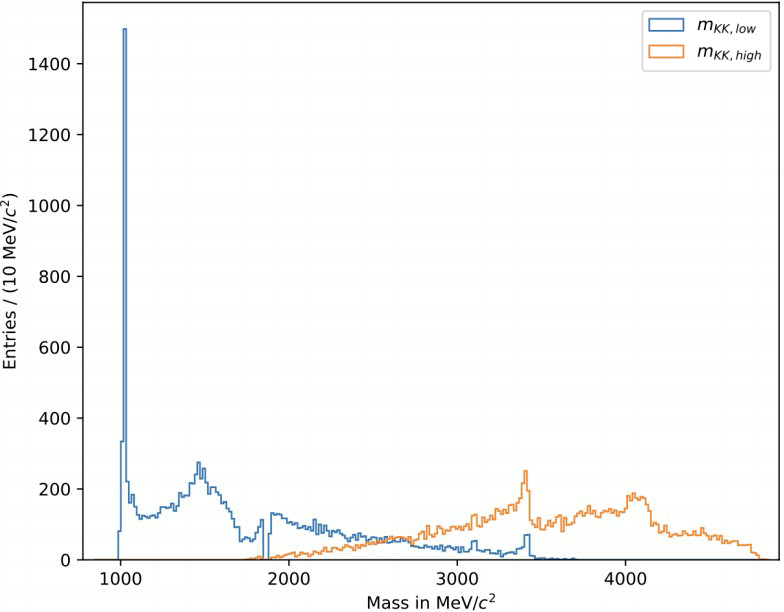
\includegraphics[width=9.2cm]{graph2.png}
    \caption{Neutral two-body invariant mass distributions of high and low mass pairs for the intermediate step $B^{\pm} \rightarrow R^{0}K^{\pm}$}
\end{figure}

Figure 2 shows multiple peaks corresponding to decays via resonance particles. We perform a mass cut of width $40 \ \mathrm{MeV}$ centered on $1865 \ \mathrm{MeV}$ to reject the charmed $D^0$ meson peak. We also identify a small $J/\psi$ meson peak at $3097 \ \mathrm{MeV}$ that decays to $\mu^{+}\mu{-}$, sufficiently suppressed due to Muon vetoing in the data selection. With our cleaned data, we find peak counts $N^{+}, N^{-} = 306, 275$, giving an initial raw estimate of CP asymmetry $A_{raw} = (-0.053 \pm 0.007) \ \mathrm{MeV}$.\newline  

We measure the $J/\psiK^{\pm}$ peak asymmetry as a control to quantify systematic uncertainty from our equipment. Measuring $N^\pm$ with a width of $20 \ \mathrm{MeV}$ centered on the peak, we get $A_{raw}(J/\psi K^{\pm}) = (−0.015 \pm 0.009) \ \mathrm{Mev}$. By subtracting the true CP Asymmetry $A_{CP}(J/\psi K^{\pm}) = (0.0018 \pm 0.0030) \ \mathrm{MeV}$ \cite{Bplusminus} we obtain a $B^{\pm}$ production asymmetry of $A_\Delta = (0.0132 \pm 0.0095) \ \mathrm{MeV}$. This is likely due to the hadronisation process during $pp$ collisions that produces the mesons, where heavy flavour production rates differ between particles and antiparticles \cite{production}. Our final $B^{\pm}$ global CP Asymmetry $A_{CP} = A_{raw} - A_{\Delta} = (-0.039 \pm 0.013) \ \mathrm{MeV}$. \newline     

\begin{figure}[htp]
    \centering
    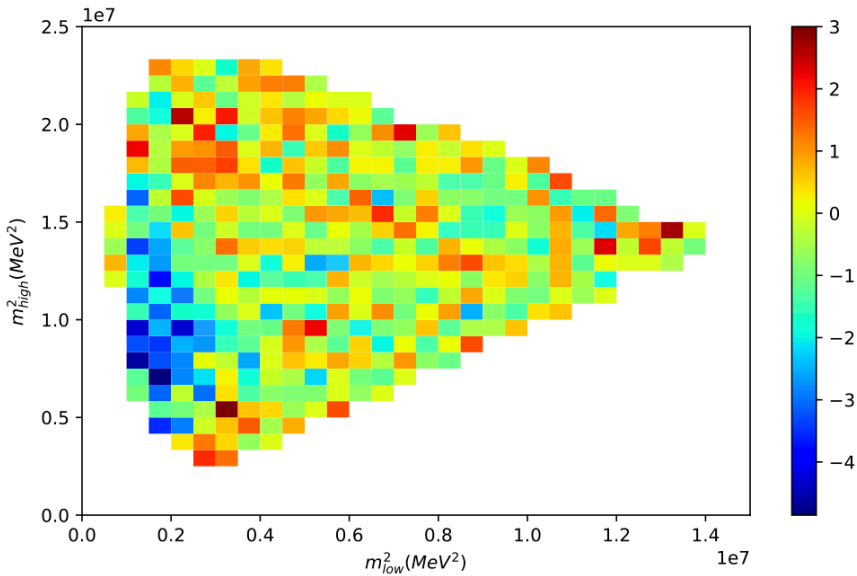
\includegraphics[width=9.2cm]{graph3.png}
    \caption{Folded Dalitz Plot for $A_{CP}$ significance, calculated as $A_{CP}/\sigma_{A_{CP}}$ per bin. Plotted against squared high and low mass pairs, after background removal and $D^0$ mass cut.}
\end{figure}
From Figure 3, we see significant negative CP Asymmetry in the $(0.1\sim0.2)\times 10^7 \ \mathrm{MeV^2}$ low mass pair range, which is consistent with the charmless resonance peaks in Figure 2. The larger peak coincides with $\phi(1020)$, and the smaller with a variety such as $\rho(1450)$. Since we model $A_{CP}$ binomially, ${\sigma_{A_{CP}}} \rightarrow 0$ as $A_{CP} \rightarrow 1$. This introduces false significant CP violations especially along the Dalitz plot boundaries, where data points per bin are low, increasing the probability of anomalous results. While we reject these events to reduce uncertainty, we see artefacts in the dark red bins around the $1.3 \times 10^7 \ \mathrm{Mev^2}$ region. We also seem them in the $(0.33\sim0.35) \times 10^7 \ \mathrm{Mev^2}$ low mass pair band, which is due the $D^0$ mass cut lowering the number of data points in those bins.

\section{Conclusions}
Our global $A_{CP} = (-0.039 \pm 0.013) \ \mathrm{MeV}$ after factoring in noise and systematic uncertainty is within 3 standard deviations of $0$. This is not significant enough to conclusively state that the decay of $B^{\pm} \rightarrow K^{\pm}K^{+}K^{-}$ globally violates CP symmetry, and would therefore have a negligible effect on the matter dominance we see in the universe. We do, however, see significant local CP violation in mass regions corresponding to resonance particles in the $(0.1\sim0.2)\times 10^7 \ \mathrm{MeV^2}$ low mass pair range. These specific particle decays could therefore have contributed in the big bang and early stages of the universe to the matter-antimatter asymmetry in the universe.

\printbibliography
\end{document}

\begin{comment}

$M_{\phi}=1020 \ \mathrm{Mev}$

$M_{\rho(1450)}=1500 \ \mathrm{Mev}$

$M_{\chi c0}=3414 \ \mathrm{Mev}$

\end{comment}